% slide 5: explaining L2R method 
% slide 6: L2R approaches
% slide 7: RankLib

\begin{frame}
  \frametitle{Learning to Rank Method}
  
  \begin{figure}[tbph]
    \centering
    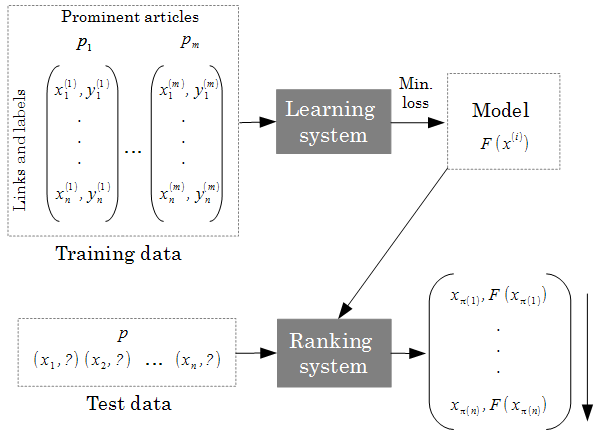
\includegraphics[width=\linewidth]{images/l2r}
  \end{figure}
  
\end{frame}

\begin{frame}
  \frametitle{L2R Approaches}
  \begin{block}{Pointwise}
   \begin{itemize}
    \item Each link is standalone instance.
    \item Input for Model: Feature Vector.
    \item Output for Model: Predicted Label.
    \item Loss Function: Based in single objects. Simplified to regression, classification, or ordinal regression.
  \end{itemize}
  \end{block}
\end{frame}

\begin{frame}
  \frametitle{L2R Approaches}
  \begin{block}{Pairwise}
   	\begin{itemize}
    	\item Considers pairs of links.
    	\item Input for Model: Pair of feature vectors.
    	\item Output for Model: Relative preference.
    	\item Loss Function: Discrepancy between preference predicted by the model and order in ground truth.
	  \end{itemize}
    \end{block}
\end{frame}

\begin{frame}
  \frametitle{L2R Approaches}
  \begin{block}{Listwise}
   	\begin{itemize}
    	\item Considers whole list of links.
    	\item Input for Model: List of feature vectors.
    	\item Output for Model: List of labels or permutation.
    	\item Loss Function: Directly measure final position/rank of links.
	  \end{itemize}
    \end{block}
\end{frame}

\begin{frame}
  \frametitle{RankLib}
  \centering
  	Library of Learning to Rank algorithms.
  \begin{figure}[tbph]
    \centering
    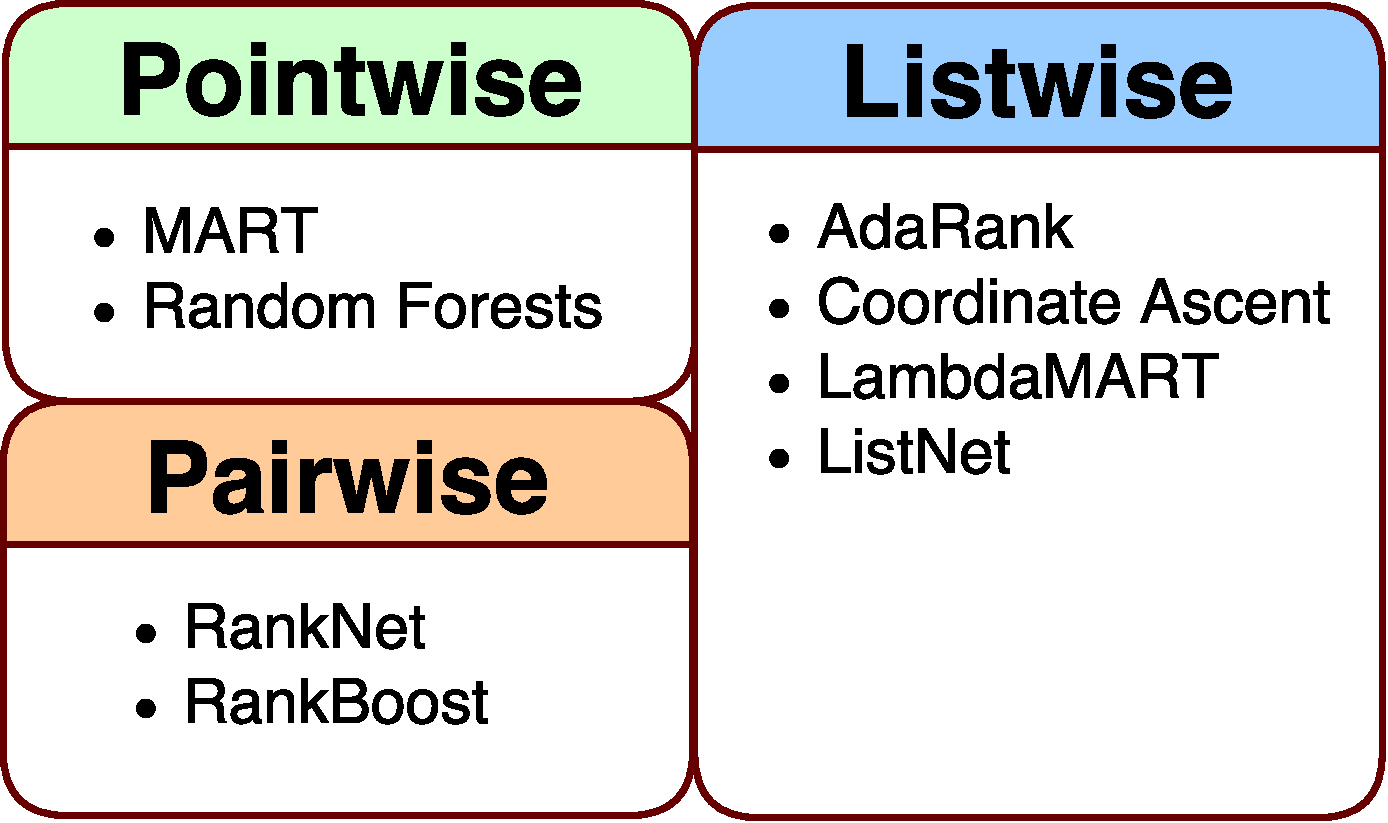
\includegraphics[width=0.7\linewidth]{images/RankLib}
  \end{figure}
\end{frame}


